\documentclass{article}

\usepackage{pgf}
\usepackage{tikz}
\usetikzlibrary{arrows,automata}
\usepackage[latin1]{inputenc}
\usepackage{verbatim}

\begin{document}

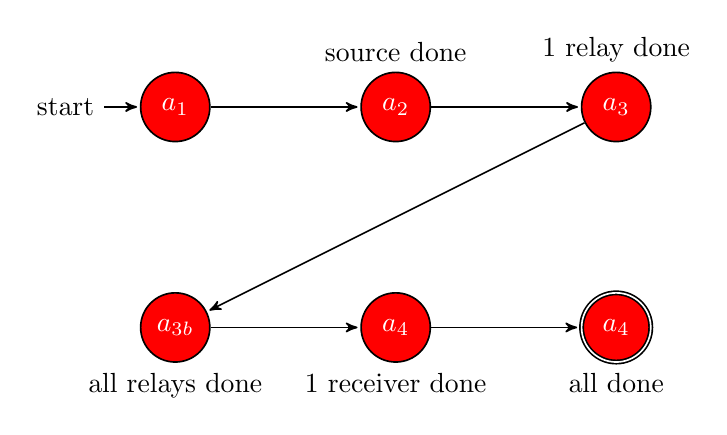
\begin{tikzpicture}[->,>=stealth',shorten >=1pt,auto,node distance=2.8cm,
                    semithick]

  %\tikzstyle{every state}=[fill=red,draw=none,text=white]
  \tikzstyle{every state}=[fill=red,text=white]

  \node[initial,state]
    (A1) {$a_1$};
  \node[state]
    (A2) [right of=A1, label=above:source done] {$a_2$};
  \node[state]
    (A3) [right of=A2, label=above:1 relay done] {$a_3$};
  \node[state]
    (A3b) [below of=A1, label=below:all relays done] {$a_{3b}$};
  \node[state]
    (A4) [below of=A2, label=below:1 receiver done] {$a_4$};
  \node[state, accepting]
    (A5) [below of=A3, label=below:all done] {$a_4$};

  \path (A1)  edge (A2)
        (A2)  edge (A3)
        (A3)  edge (A3b)
        (A3b) edge (A4)
        (A4)  edge (A5);

\end{tikzpicture}

\end{document}
